The transport proxy's job is to negotiate and convert the media streams to allow for interoperation between WebRTC and enterprise communication endpoints. The specific problems related to this component are repeated below:

\begin{itemize}
\item{How to implement ICE?}
\item{How to negotiate the DTLS secret keys?}
\item{How to decrypt and encrypt the media streams from SRTP to RTP and reverse?}
\item{How to handle multiplexing and demultiplexing of the streams?}
\end{itemize}

%test web breaker for stun turn - look at ice candidates
%i'm not describing or testing crypto - why?
%dtls is basically tls for udp - won't go into that or the encryption/decryption part
%not looking for multiplexing in web breaker -why? Wireshark does not have great handling show screenshot/no rtcp) was not able to resolve packets as one rtcp stream

We could either roll or own implementation or re-use the RTCWeb Breaker from the previous chapter for this component. If we create our own transport proxy, we could either use Google's libjingle library\footnote{https://code.google.com/p/libjingle/}, which is an open-source C++ library for doing peer-to-peer applications, or implement or own solution for doing ICE negotiations. The point is we need to speak the STUN and TURN protocols. For incoming streams we should block all non-relayed streams in the firewall and use TURN for realying the media flows, but for outgoing streams we should be able to use STUN and deliver the streams directly to the WebRTC peer if possible. After we have handled ICE, we need to translate the media flows. VA communicates RTP media and RTCP control flows, both of these needs to have their packets encrypted. We do this by running a DTLS handshake that establishes a shared secret key between the peers, which is then reused as keying material within SRTP and SRTCP. Lastly, both SRTP and SRTCP requires to run on separate ports for each individual stream, which is a problem for clients running behind NATs and firewalls. Therefore we must support both multiplexing and demultiplexing of the streams in this component. This allows us to enable delivery of multiple streams and control channels on the same destination port.

By looking at the results of the experiments using RTCWeb Breaker introduced in the previous chapter, we can see that there was not much problems in this module, the connections were smooth with low latency, even running behind a proxy the connection felt `live'. The RTCWeb Breaker seems to work exactly as it should. As mentioned earlier there was no problems doing audio calls, but video calling seemed to cause some problems, this is probably not related to this component, since audio runs over the same protocols as video. It is probably to do with the clients not being able to agree on a common video codec. In Figure \ref{fig:wireshark-sip-call-flow} we can see an anlysis of the SIP call flow. We can see the call setup and the codecs which were offered. The codec used in this case was g.711 for audio. Lastly there is an acknowledgement of the hang up.

\begin{figure}[here]
\centerline{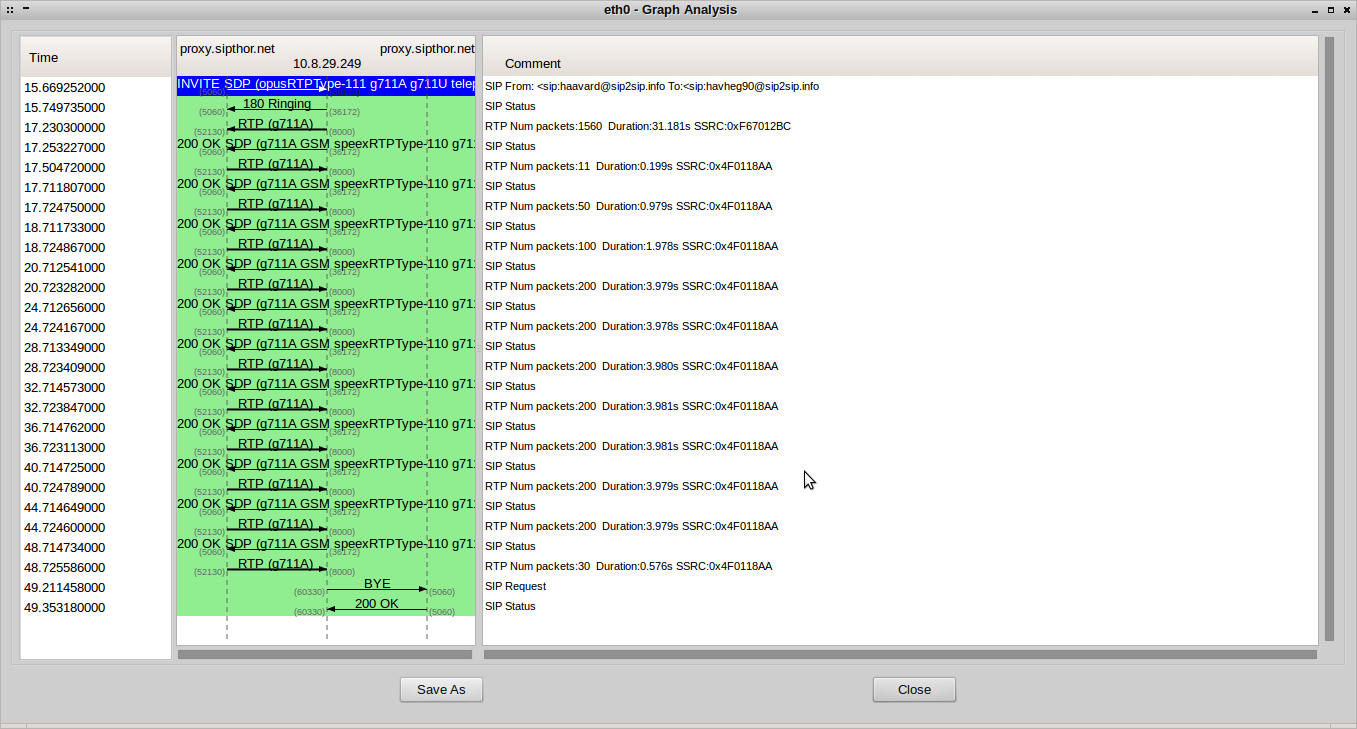
\includegraphics[scale=0.25]{call-flow.png}}
\caption{Wireshark SIP call flow}
\label{fig:wireshark-sip-call-flow}
\end{figure}

There could theoretically be a firewall issue, but this is highly doubtable since audio worked perfectly well in all cases, and \gls{rtcweb} supports multiplexing of the media streams, so they should be running over one single port if there was a firewall limitation. The calling in all cases was pretty much instant with very little delay, this means that ICE found working candidates really fast, even when testing behind a proxy.

\section{Summary}
The \gls{wrtc} specification make support for \gls{ice} and \gls{srtp}-{dtls} mandatory. The problem here is that our enterprise architecture uses raw \gls{rtp} streams, it does not need the added transport layer security that \gls{wrtc} defines, becuse of its strict firewall policies. It is up to the Transport Proxy to add and remove security to the media streams for allowing these two worlds to interoperate. The Transport Proxy also has to modify the ICE transport object to use a TURN server, this so we can bypass our firewall. In addition we need to multiplex the streams so that they can run over the same port.